% ════════════════════════════════════════════
% 模型求解（5.2.4）
% ════════════════════════════════════════════
\subsubsection{结果与解读}

基于上述规则，本节对 500 条帖子逐项执行清洗与编码，并把结果写入统一分析数据。求解环境为 Python 3，使用 pandas 完成缺失统计、类别编码与变换，使用 SciPy 完成分布指标计算。

首先给出缺失与异常核查结果。由表\ref{tab:q2_check}可知，7 个输入变量的取值范围全部落在字段说明之内，没有越界值，也没有完全重复的帖子。唯一缺失出现在 X7，已按众数填补；X6 的 0 时与 21 时没有帖子，实际只有 22 个取值；Y1 的 1,110,282 次是一条真实的病毒式传播记录，不作删除，改由 log1p 变换压缩其影响。

\begin{longtable}{>{\centering\arraybackslash}p{0.19\textwidth}>{\centering\arraybackslash}p{0.31\textwidth}>{\centering\arraybackslash}p{0.23\textwidth}>{\centering\arraybackslash}p{0.15\textwidth}}
  \caption{缺失与异常检查}
  \label{tab:q2_check} \\
  \toprule
  检查项 & 实际结果 & 判断 & 处理 \\
  \midrule
  \endfirsthead
  \caption{缺失与异常检查（续）} \\
  \toprule
  检查项 & 实际结果 & 判断 & 处理 \\
  \midrule
  \endhead
  \bottomrule
  \endfoot
  X1 取值范围 & 81,370 至 139,441 & 在字段说明范围内 & 保留 \\
  X2 取值集合 & Photo、Status、Link、Video & 4 类，与说明一致 & 转为名义变量 \\
  X3 取值集合 & 1、2、3 & 3 类，与说明一致 & 转为名义变量 \\
  X4 取值范围 & 1 至 12 & 无越界 & 保留并编码 \\
  X5 取值范围 & 1 至 7 & 无越界 & 保留并编码 \\
  X6 取值范围 & 样本 1 至 23，0 时与 21 时无帖子 & 落在 0 至 23 内 & 按分布合并为 3 组 \\
  X7 取值集合 & 0、1，缺失 1 条 & 二元变量，第 499 行缺失 & 众数填补，另做删除对照 \\
  Y1 取值范围 & 570 至 1,110,282 & 全部为正，与说明一致 & log1p 变换 \\
  完全重复行 & 0 条 & 无重复帖子 & 无需去重 \\
  异常值 & 1 条 1,110,282 次的极端曝光 & 属真实传播事件，非录入错误 & 保留，由变换压缩 \\
  缺失填补 & 众数 0，共 1 条 & 填补后无缺失 & 保留填补标记 \\
\end{longtable}

表\ref{tab:q2_scheme}汇总了编码与变换方案。连续变量 X1 取对数，计数型因变量 Y1 取 log1p；名义变量 X2、X3 分别以 Photo、主题 1 为参照；月份、星期保留全部哑变量；时段合并为三组并以上午为参照；X7 保持 0/1 数值。该方案共产生 26 个参数，与最终回归模型一致。

\begin{longtable}{>{\centering\arraybackslash}p{0.10\textwidth}>{\centering\arraybackslash}p{0.14\textwidth}>{\centering\arraybackslash}p{0.20\textwidth}>{\centering\arraybackslash}p{0.14\textwidth}>{\centering\arraybackslash}p{0.26\textwidth}}
  \caption{编码与变换方案}
  \label{tab:q2_scheme} \\
  \toprule
  变量 & 识别类型 & 编码或变换 & 基线或参照 & 解释 \\
  \midrule
  \endfirsthead
  \caption{编码与变换方案（续）} \\
  \toprule
  变量 & 识别类型 & 编码或变换 & 基线或参照 & 解释 \\
  \midrule
  \endhead
  \bottomrule
  \endfoot
  X1 & 连续 & $\log(X_1)$ & 无 & 粉丝规模弹性，压缩量级 \\
  X2 & 名义，4 类 & 独热编码，3 个哑变量 & Photo & 相对图片的曝光差异 \\
  X3 & 名义，3 类 & 独热编码，2 个哑变量 & 主题 1 & 相对主题 1 的曝光差异 \\
  X4 & 有序，12 类 & 独热编码，11 个哑变量 & 1 月 & 控制季节性与时间趋势 \\
  X5 & 有序，7 类 & 独热编码，6 个哑变量 & 周一 & 控制星期效应 \\
  X6 & 有序，24 类 & 合并 3 组，2 个哑变量 & 上午 & 控制时段效应，避免稀疏 \\
  X7 & 二元 & 0/1 数值 & 0，自然 & 付费的额外曝光 \\
  Y1 & 连续计数 & $\log(1+Y_1)$ & 无 & 压缩重尾，系数近似百分比 \\
\end{longtable}

变换效果由表\ref{tab:q2_trans}给出。曝光量偏度由 8.3259 降至 0.7341，峰度由 93.0526 降至 0.8209，两项指标都回到接近正态的范围；最小值与最大值保持不变，说明变换没有删改任何观测。粉丝规模取对数后偏度由 $-0.9795$ 变为 $-1.1541$，左偏略有加强，这是粉丝数在高位堆积的必然结果，但其量级跨度被显著压缩，有利于数值稳定。

\begin{longtable}{>{\centering\arraybackslash}p{0.10\textwidth}>{\centering\arraybackslash}p{0.11\textwidth}>{\centering\arraybackslash}p{0.11\textwidth}>{\centering\arraybackslash}p{0.11\textwidth}>{\centering\arraybackslash}p{0.11\textwidth}>{\centering\arraybackslash}p{0.11\textwidth}>{\centering\arraybackslash}p{0.11\textwidth}}
  \caption{变换前后分布特征}
  \label{tab:q2_trans} \\
  \toprule
  变量 & 偏度（前） & 偏度（后） & 峰度（前） & 峰度（后） & 最小值 & 最大值 \\
  \midrule
  \endfirsthead
  \caption{变换前后分布特征（续）} \\
  \toprule
  变量 & 偏度（前） & 偏度（后） & 峰度（前） & 峰度（后） & 最小值 & 最大值 \\
  \midrule
  \endhead
  \bottomrule
  \endfoot
  Y1 & 8.3259 & 0.7341 & 93.0526 & 0.8209 & 570 & 1110282 \\
  X1 & $-0.9795$ & $-1.1541$ & $-0.2759$ & 0.1845 & 81370 & 139441 \\
\end{longtable}

表\ref{tab:q2_missing}报告缺失处理的敏感性。众数填补下付费系数为 0.3374，删除缺失行后为 0.3363，两者相差 0.0011，远小于预设的 0.01 阈值；标准误分别为 0.1115 与 0.1117，样本量分别为 500 与 499。可见填补方案既不改变系数方向，也不改变显著性判断，后续分析可以放心使用填补后的 500 条样本。

\begin{longtable}{>{\centering\arraybackslash}p{0.40\textwidth}>{\centering\arraybackslash}p{0.16\textwidth}>{\centering\arraybackslash}p{0.16\textwidth}>{\centering\arraybackslash}p{0.16\textwidth}}
  \caption{缺失处理敏感性}
  \label{tab:q2_missing} \\
  \toprule
  方案 & 付费系数 & 标准误 & 样本量 \\
  \midrule
  \endfirsthead
  \caption{缺失处理敏感性（续）} \\
  \toprule
  方案 & 付费系数 & 标准误 & 样本量 \\
  \midrule
  \endhead
  \bottomrule
  \endfoot
  众数填补 & 0.3374 & 0.1115 & 500 \\
  删除缺失行 & 0.3363 & 0.1117 & 499 \\
  差异 & 0.0011 & 无 & 无 \\
\end{longtable}

如图\ref{fig:q2_cat}所示，类别结构存在明显的不平衡。帖子类型中 Photo 有 426 条，占绝对多数，Status 45 条、Link 22 条、Video 仅 7 条；内容主题三类的数量分别为 215、130、155，相对均衡；付费标记在填补后为自然 361 条、付费 139 条，另有 1 条原始缺失。发帖小时呈双峰分布，凌晨 3 时最多（105 条），上午 10 时次之（78 条），合并后的凌晨、上午、下午晚间三组分别为 196、193、111 条。视频类型与链接类型的样本量提示其估计精度有限，这一限制将在效应测算的区间宽度中直接体现。

\begin{figure}[ht]
  \centering
  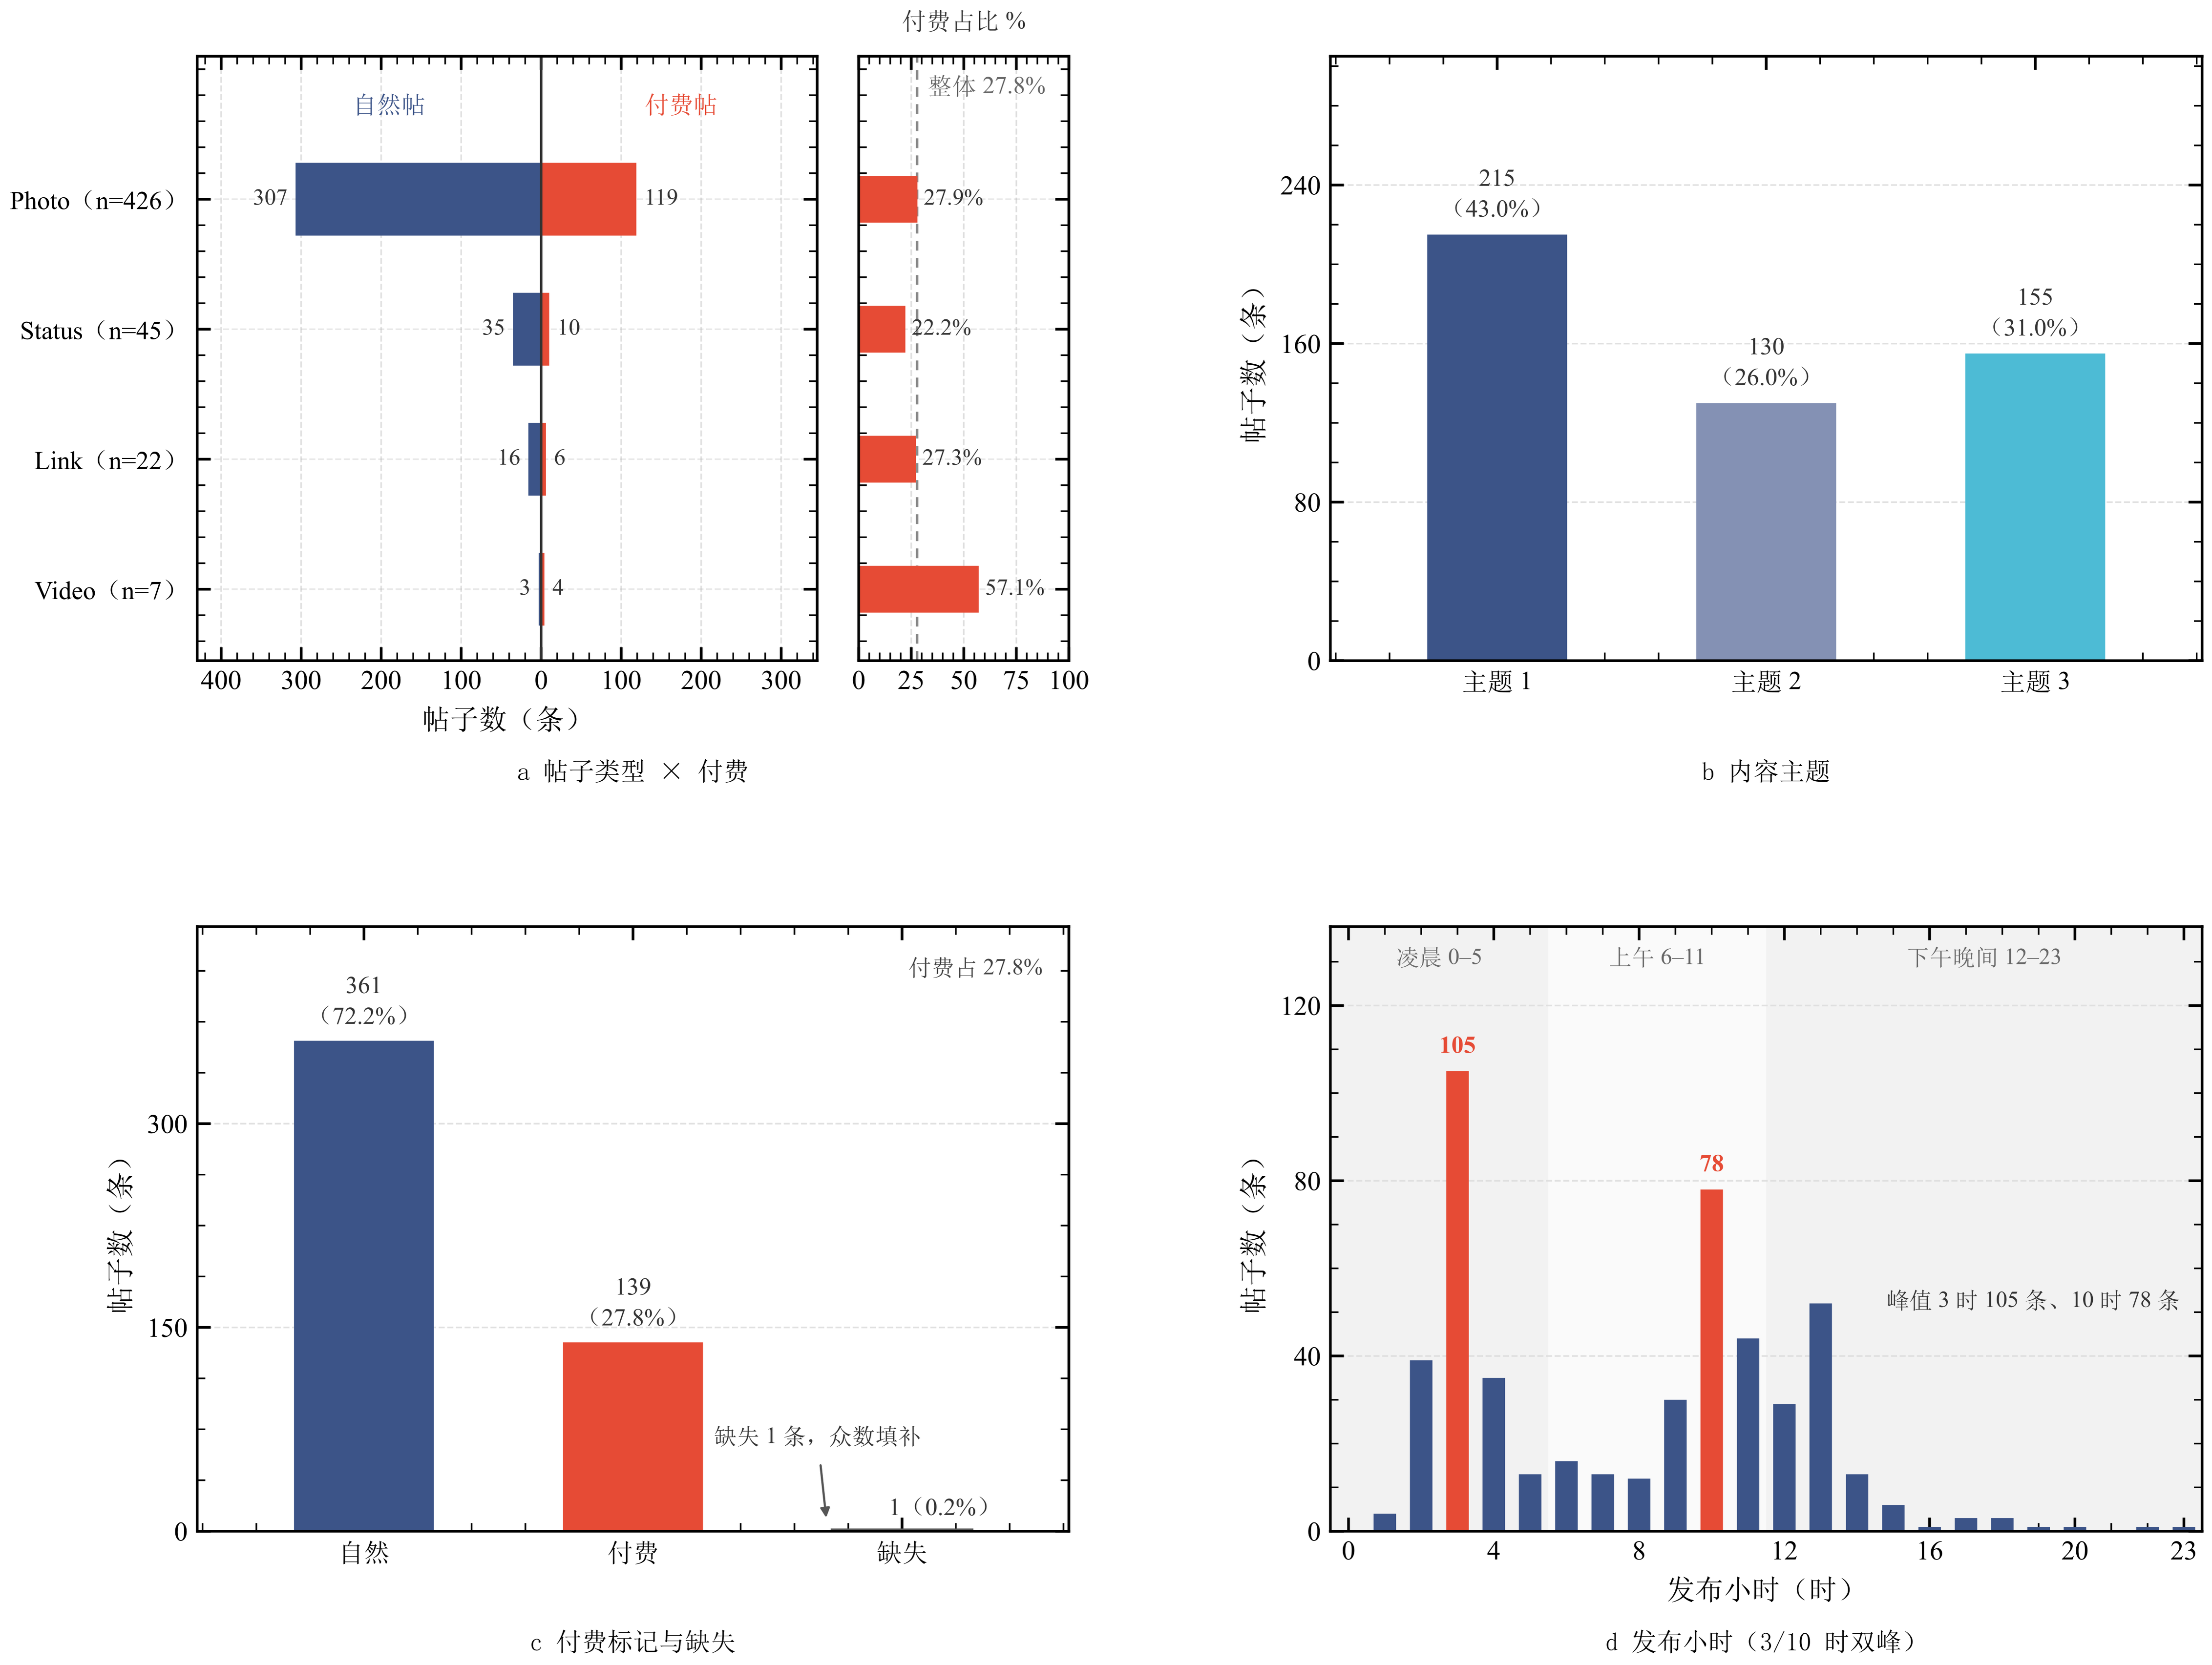
\includegraphics[width=0.68\textwidth]{../求解/问题二/结果/图4_类别结构与缺失.png}
  \caption{类别结构与缺失分布}
  \label{fig:q2_cat}
\end{figure}

图\ref{fig:q2_trans}从分布形态与分位数两个角度对比变换效果。原始曝光量的直方图在 30 个等宽区间内有 414 条帖子落入首个区间，占 82.8\%，其余观测拖出长尾；log1p 变换后的密度曲线与正态密度接近重合，Q--Q 图上的点也基本沿参考线分布，仅两端略有偏离。这说明 log1p 既保留了样本排序，又把极端值拉回了可建模的范围。

\begin{figure}[ht]
  \centering
  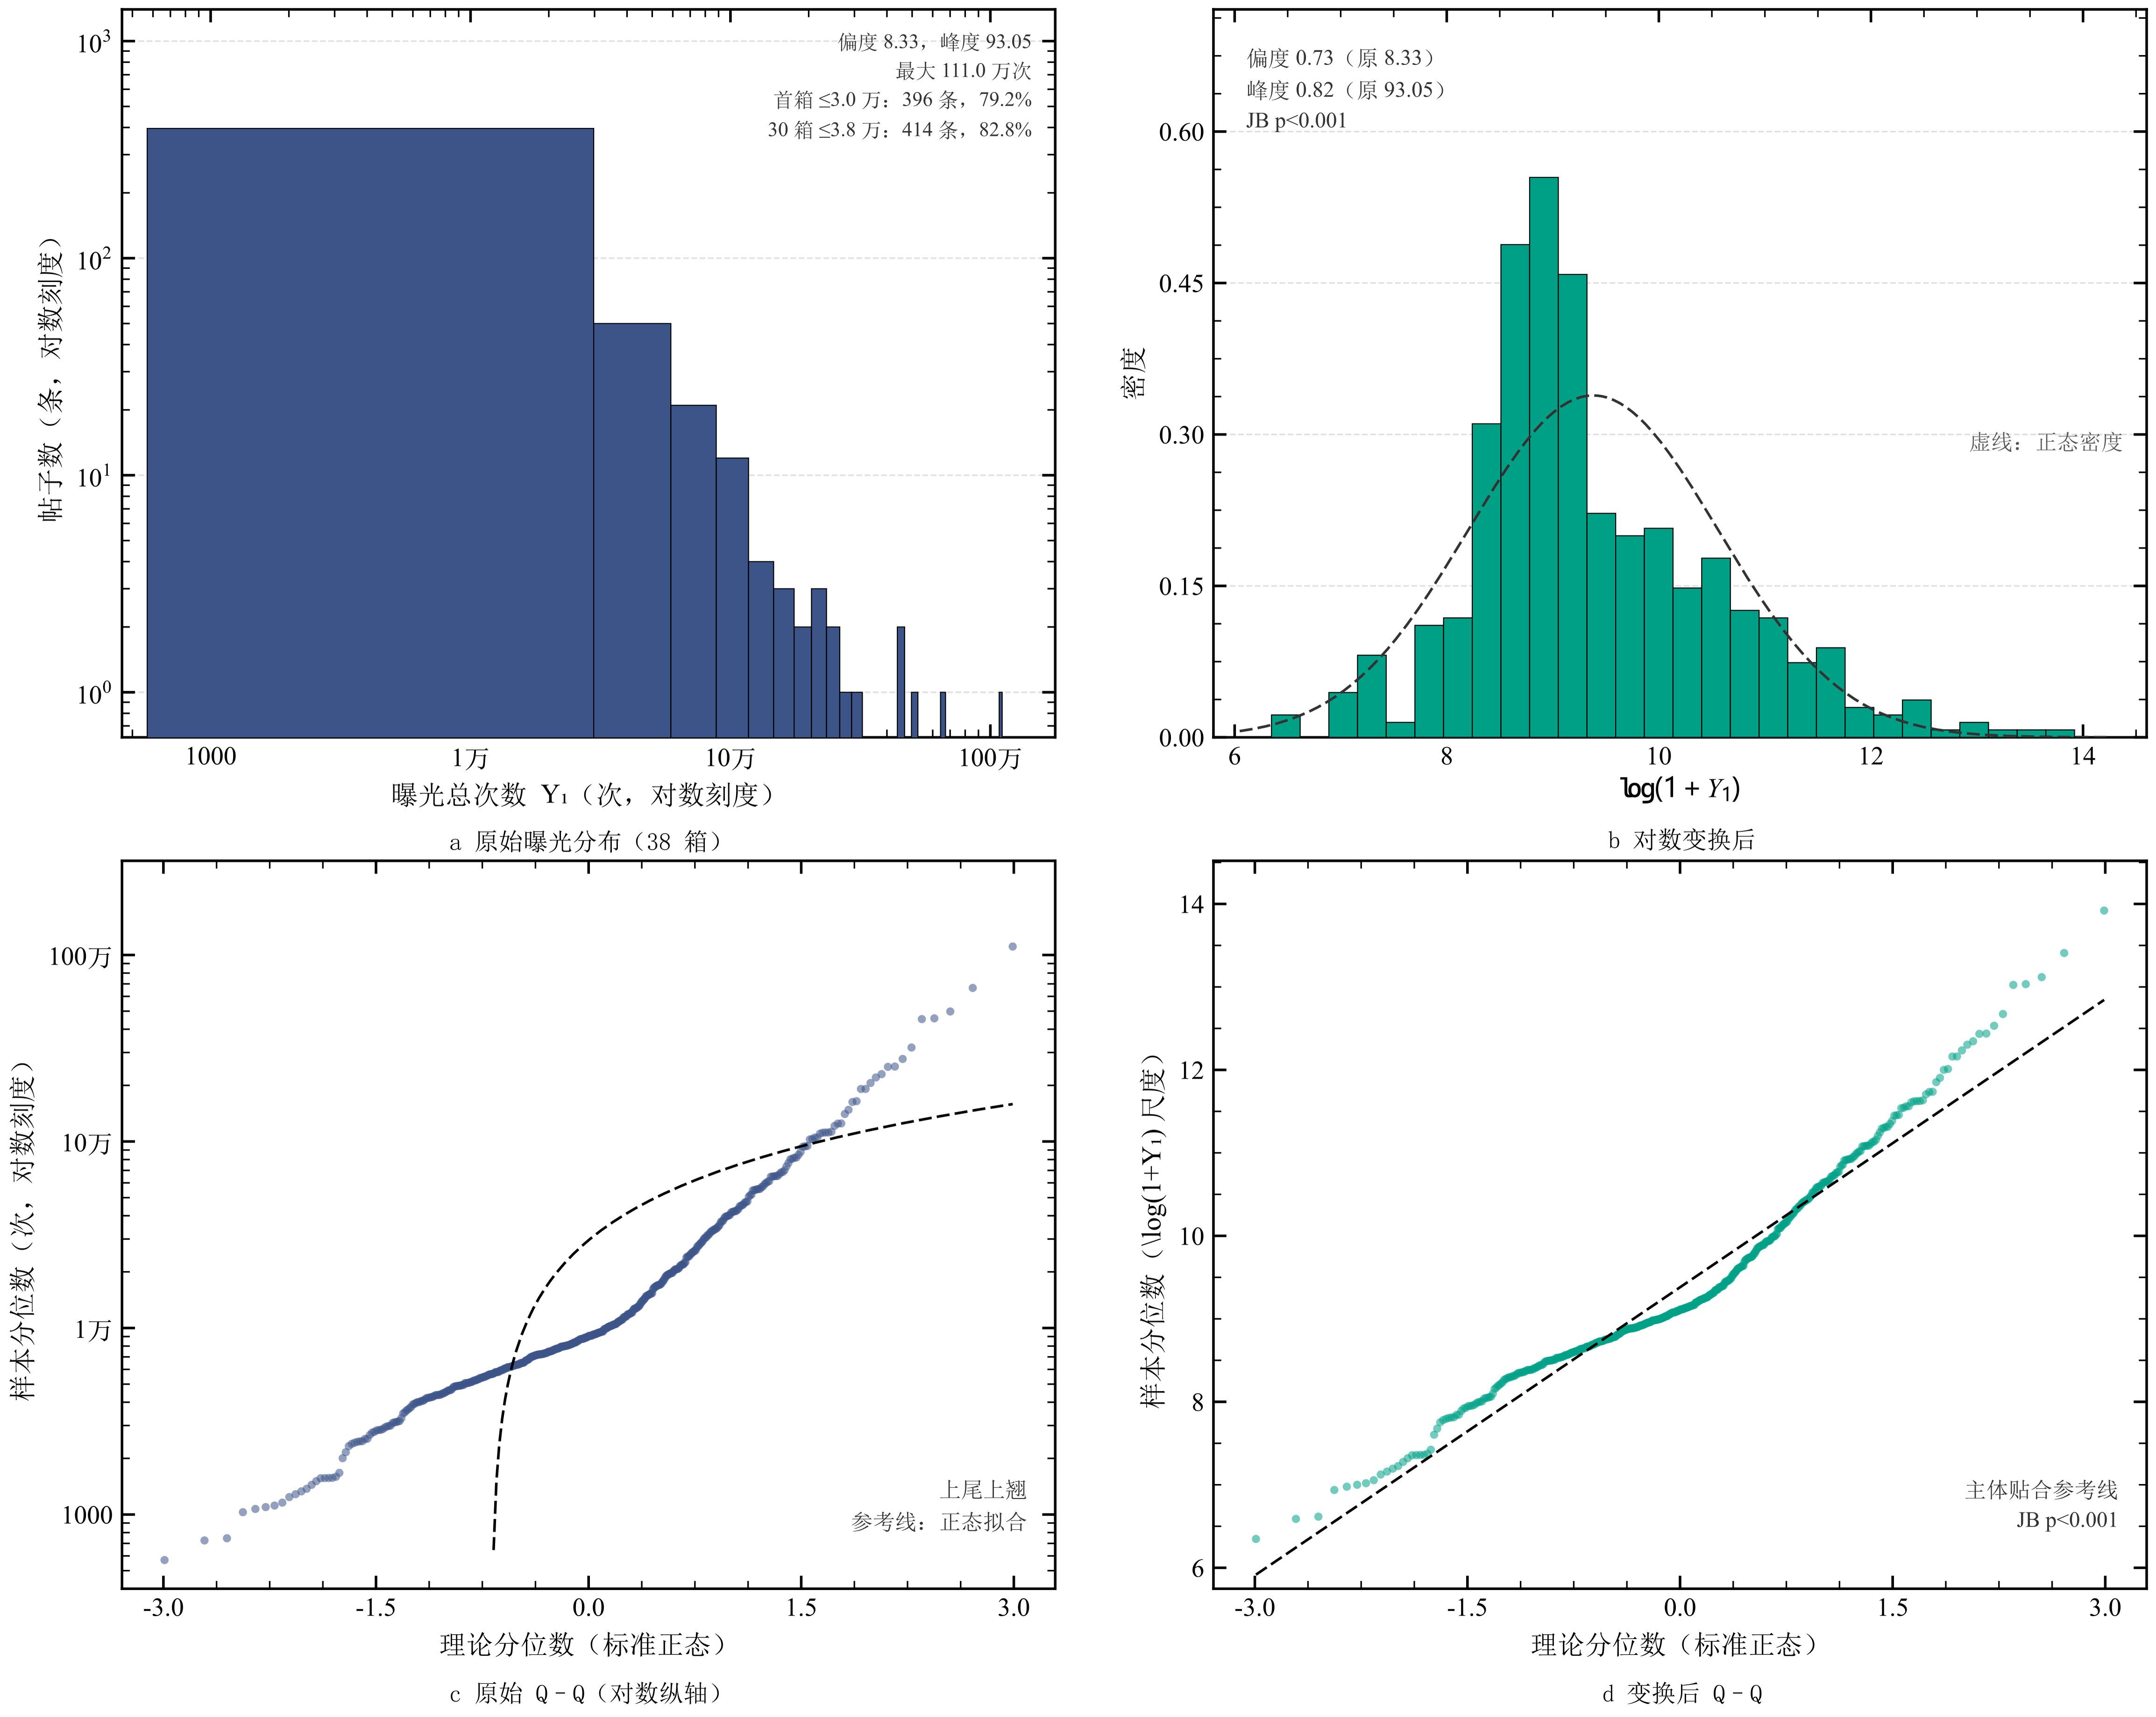
\includegraphics[width=0.68\textwidth]{../求解/问题二/结果/图5_变换前后分布.png}
  \caption{曝光量变换前后的分布与 Q--Q 图}
  \label{fig:q2_trans}
\end{figure}

在完成编码前，图\ref{fig:q2_time}先核对时间变量的经验结构。左上图把逐月发帖量与付费占比放在双轴上：发帖量在 1 月最低（25 条）、10 月最高（60 条），付费占比在 1 月的 16.0\% 与 4 月的 40.0\% 之间波动，既没有单边趋势，也不与发帖量同步。右上图给出逐月平均对数曝光的 95\% 置信带，2 月最高（10.13）、10 月最低（8.83），两月区间不重叠，说明月份既承载账号成长，也混入季节性的内容表现。左下图按星期排列，周四均值最高（9.74）、周日最低（9.06）；右下图按合并后的时段排列，上午最低（9.25）、下午晚间最高（9.50）。不过，星期与时段在控制月份、类型与主题后均不再显著（时段系数的 $p$ 值为 0.145 与 0.655），原始差异主要来自内容构成而非发布时间本身。基于这组证据，月份与星期保留为固定效应，24 小时合并为凌晨、上午、下午晚间三组，以避免稀疏小时带来不稳定估计。

\begin{figure}[ht]
  \centering
  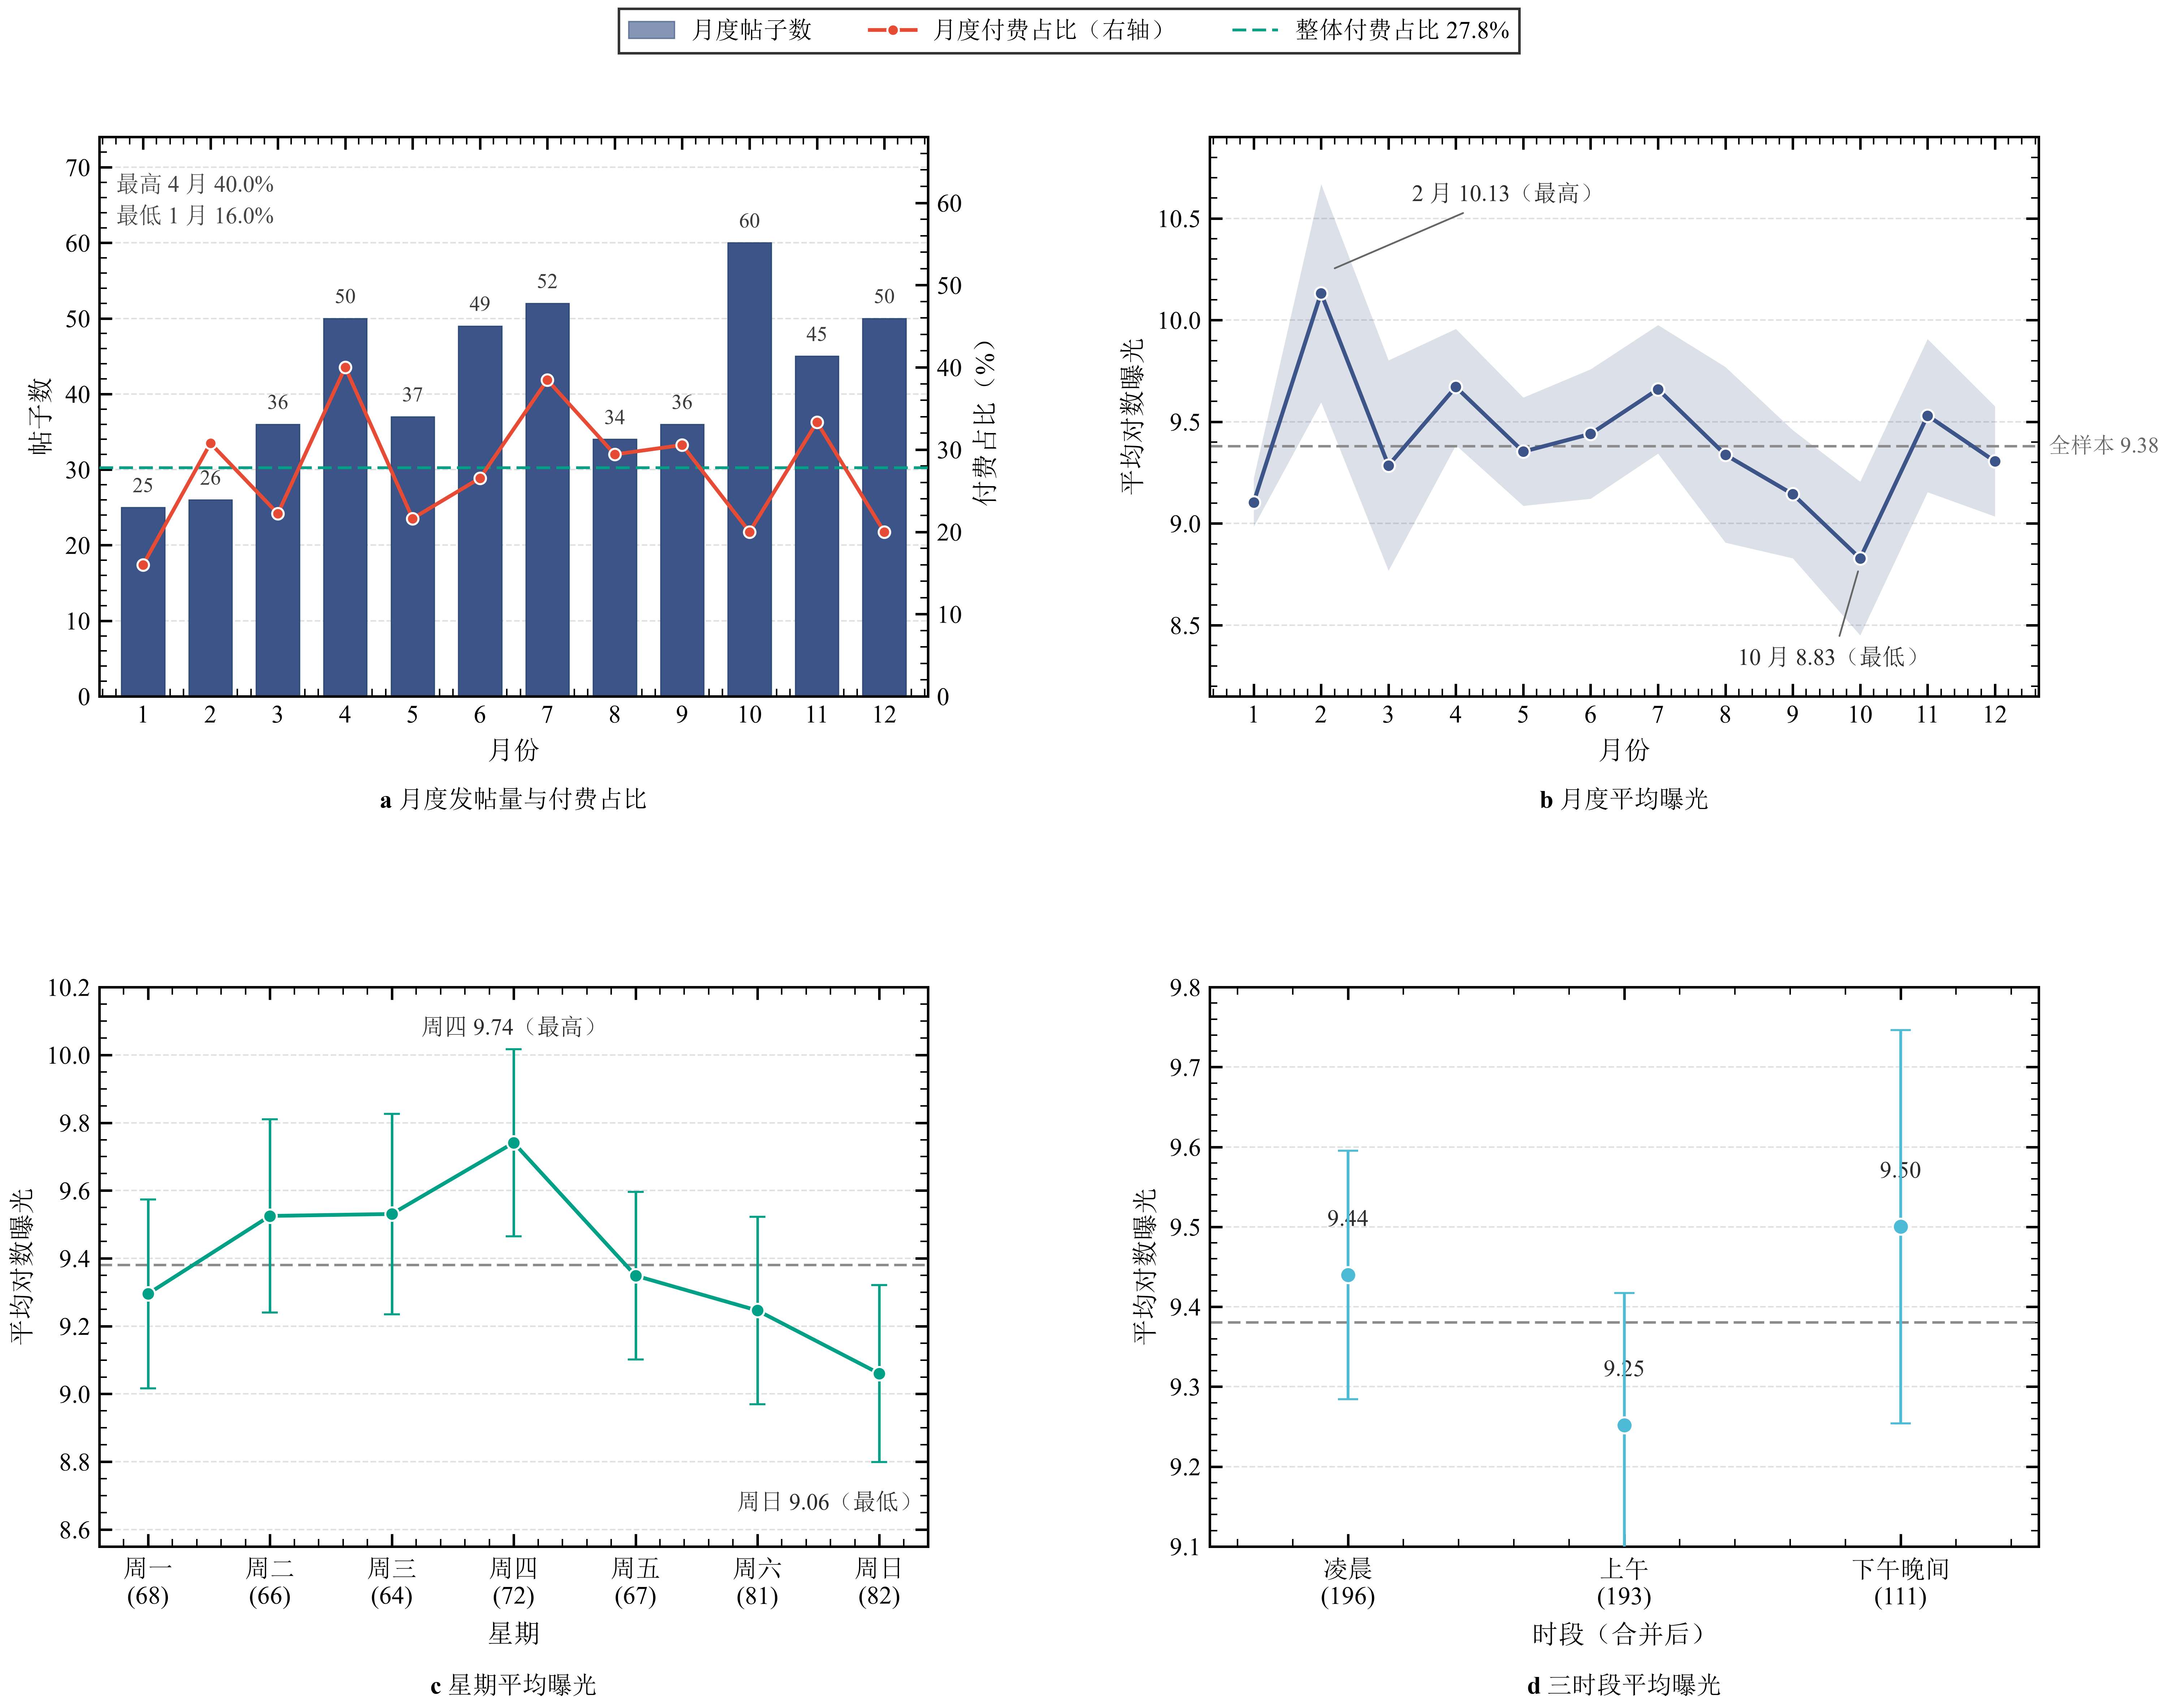
\includegraphics[width=0.80\textwidth]{../求解/临时产物/补充图2_时间结构.png}
  \caption{发帖量、付费占比与曝光的时间结构}
  \label{fig:q2_time}
\end{figure}

综合以上结果，清洗后的数据无缺失、无重复、无越界，类别编码完整，曝光量分布接近对称，缺失处理方案对系数的影响仅 0.0011。统一分析数据共 500 行，包含原始列、编码列、变换列与填补标记，可直接供回归建模与效应测算复用。
